\documentclass[border=5pt]{standalone}
\usepackage[T1]{fontenc}\usepackage{lmodern}\usepackage{pgfplots}
\usepgfplotslibrary{groupplots}\pgfplotsset{compat=1.18}
\begin{document}\sffamily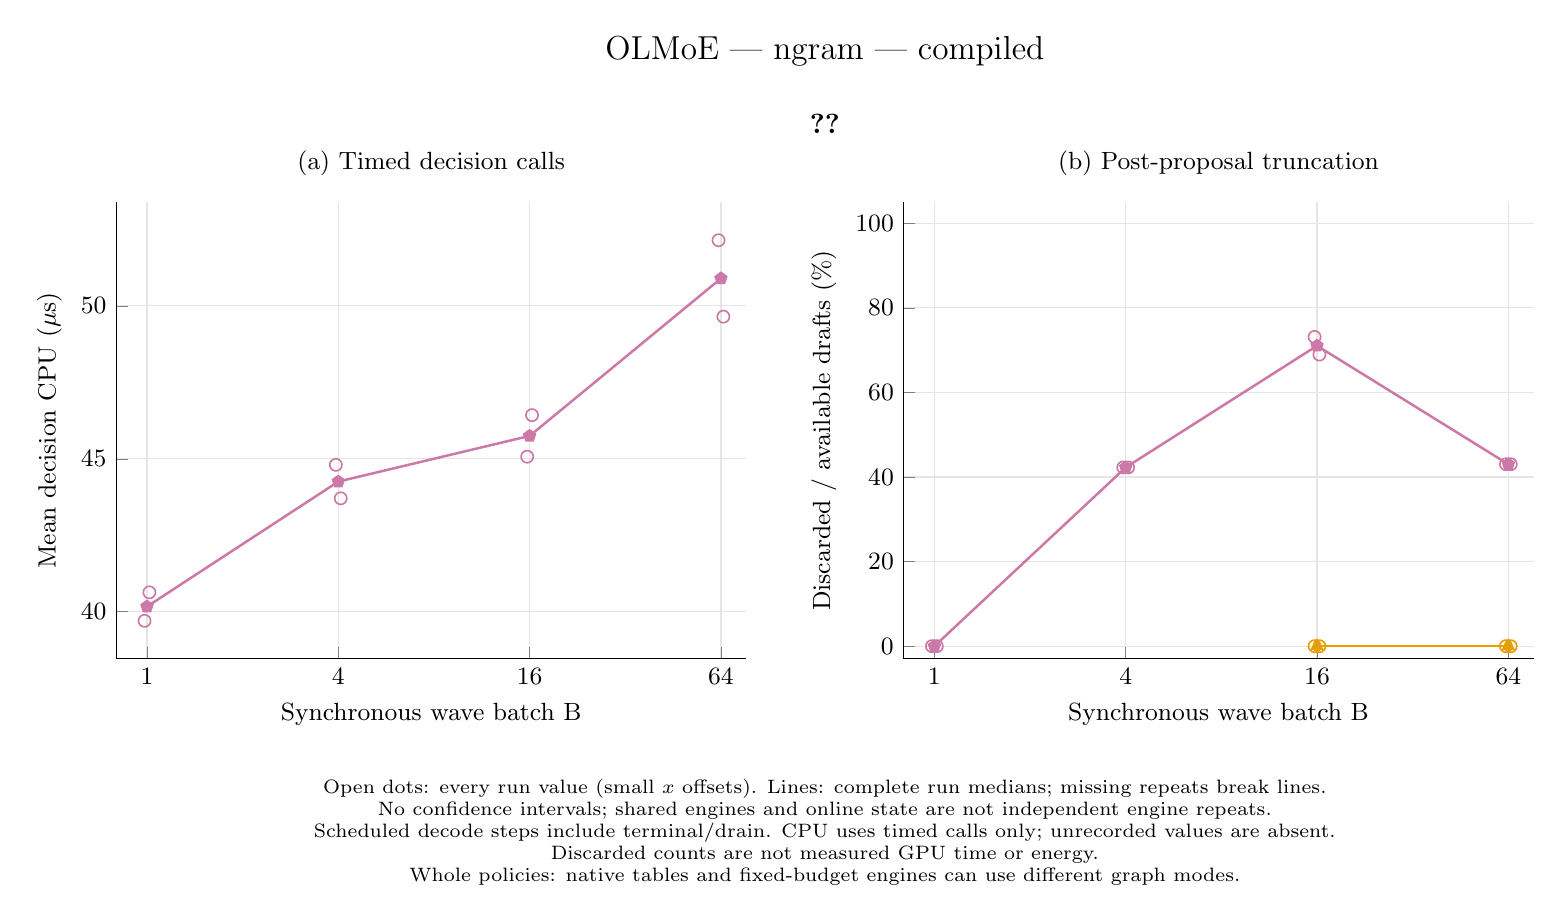
\begin{tikzpicture}
\definecolor{policy0}{HTML}{222222}
\definecolor{policy1}{HTML}{0072B2}
\definecolor{policy2}{HTML}{E69F00}
\definecolor{policy3}{HTML}{009E73}
\definecolor{policy4}{HTML}{CC79A7}
\begin{groupplot}[group style={group size=2 by 1,horizontal sep=2.0cm},width=8.0cm,height=5.8cm,scale only axis,grid=major,grid style={gray!20},axis lines*=left,unbounded coords=jump,xmode=log,log basis x=2,minor x tick num=0,scaled y ticks=false,tick label style={font=\small},label style={font=\small},title style={font=\small},xtick={1,4,16,64},xticklabels={1,4,16,64},xlabel={Synchronous wave batch B}]
\nextgroupplot[title={(a) Timed decision calls},ylabel={Mean decision CPU ($\mu$s)},xmin=0.8,xmax=76.8,legend to name=policyLegend,legend columns=3,legend style={draw=none,font=\small,/tikz/every even column/.append style={column sep=8pt}}]
\addlegendimage{color=policy2,mark=triangle*,line width=0.9pt}\addlegendentry{Native table}
\addlegendimage{color=policy4,mark=pentagon*,line width=0.9pt}\addlegendentry{Adaptive}
\addplot[forget plot,color=policy4,mark=pentagon*,mark size=2pt,line width=0.9pt] coordinates {(1,40.1698112725) (4,44.2546752844) (16,45.7473662864) (64,50.8934212598)};
\addplot[only marks,forget plot,color=policy4,mark=o,mark size=2.2pt,mark options={fill=white,line width=0.6pt}] coordinates {(0.982652235665,39.7046149378) (1.01765402215,40.6350076072) (3.93060894266,44.8017776629) (4.0706160886,43.7075729059) (15.7224357706,45.068515873) (16.2824643544,46.4262166998) (62.8897430826,52.1422204724) (65.1298574176,49.6446220472)};
\nextgroupplot[title={(b) Post-proposal truncation},ylabel={Discarded / available drafts (\%)},xmin=0.8,xmax=76.8,ymin=-3,ymax=105]
\addplot[forget plot,color=policy2,mark=triangle*,mark size=2pt,line width=0.9pt] coordinates {(1,nan) (4,nan) (16,0) (64,0)};
\addplot[only marks,forget plot,color=policy2,mark=o,mark size=2.2pt,mark options={fill=white,line width=0.6pt}] coordinates {(15.7224357706,0) (16.2824643544,0) (62.8897430826,0) (65.1298574176,0)};
\addplot[forget plot,color=policy4,mark=pentagon*,mark size=2pt,line width=0.9pt] coordinates {(1,0) (4,42.2666259915) (16,71.0463999324) (64,43.0243024302)};
\addplot[only marks,forget plot,color=policy4,mark=o,mark size=2.2pt,mark options={fill=white,line width=0.6pt}] coordinates {(0.982652235665,0) (1.01765402215,0) (3.93060894266,42.2666259915) (4.0706160886,42.2666259915) (15.7224357706,73.1300770123) (16.2824643544,68.9627228525) (62.8897430826,43.0243024302) (65.1298574176,43.0243024302)};
\end{groupplot}
\path (group c1r1.north west) -- node[above=1.6cm,font=\large] {OLMoE | ngram | compiled} (group c2r1.north east);
\path (group c1r1.north west) -- node[above=0.75cm] {\ref{policyLegend}} (group c2r1.north east);
\path (group c1r1.south west) -- node[below=1.4cm,align=center,font=\scriptsize] {Open dots: every run value (small $x$ offsets). Lines: complete run medians; missing repeats break lines.\\No confidence intervals; shared engines and online state are not independent engine repeats.\\Scheduled decode steps include terminal/drain. CPU uses timed calls only; unrecorded values are absent.\\Discarded counts are not measured GPU time or energy.\\Whole policies: native tables and fixed-budget engines can use different graph modes.} (group c2r1.south east);
\end{tikzpicture}\end{document}
